	The genome, or complete DNA sequence, of an individual consists of an ordered sequence of nucleotides (A,C,G,T). The total length of this sequence in a human genome is approximately six billion letters \cite{pevsner2015bioinformatics}. Humans are diploid species --meaning they have two copies of their genome and receive one copy from each parent. In a human organism, each cell contains a copy of the organism's genome, which is replicated through the process of cell division. As DNA molecules replicate, changes in the DNA sequence \textemdash genetic variants\textemdash  may occur. Most of the time, genetic variations have no effect at all. However, sometimes the effect of these changes may be harmful and may be passed on from one generation to the next. Structural variants (SVs), a type of genetic variant characterized by insertions, deletions, inversions, etc., of $>50$ letters,  are rare occurrences of DNA rearrangements which can provide great insights into regulation of gene expression, ethnic diversity, large-scale chromosome evolution, and their role in disease susceptibility \cite{pevsner2015bioinformatics}, \cite{SPENCE202061}, \cite{kosugi2019comprehensive}. 
	
	The common approach for SV prediction from sequencing data has been to map the resulting sequences to a reference genome and computationally identify statistically significant deviations from the expected mapping signals consistent with each class of SV \cite{lander1988genomic}. However, errors in both the sequencing and mapping process itself may cause inconsistencies in the data that falsely suggest the presence of an SV. As such, many computational approaches for SV detection suffer from high false-positive rates  \cite{lander1988genomic}, \cite{medvedev2009computational}. Despite the fact that the rate of novel germline SV is negligible \cite{genome2014whole}, and therefore any SV present in a child must have been inherited from one of their parents, most computational SV pipelines consider only one individual at a time \cite{chen2009breakdancer}, \cite{rausch2012delly}, \cite{quinlan2010genome}.
%	In addition, despite the fact that for each SV an individual carries either 1 copy (heterozygous) or 2 copies (homozygous), most computational approaches do not distinguish between these two cases (see Fig. 1). Finally, despite the fact that the rate of novel germline SV is negligible [5], and therefore any SV present in a child must have been inherited from one of their parents, most computational SV pipelines consider only one individual at a time [9], [10], [11].

	In this work, we develop a computational framework for predicting the presence of SVs by simultaneously analyzing related individuals, specifically a parent and a child. We utilize a likelihood-based approach for predicting the most likely SVs present in each individual’s genome and constrain the space of possible predictions by those that are consistent with Mendelian inheritance \cite{alliance2010understanding}. We further enforce sparsity in our predictions through an $\ell_1$ penalty term.
%	\begin{figure}[htb]
		
%	\begin{minipage}[b]{1.0\linewidth}
%		\centering
%		\centerline{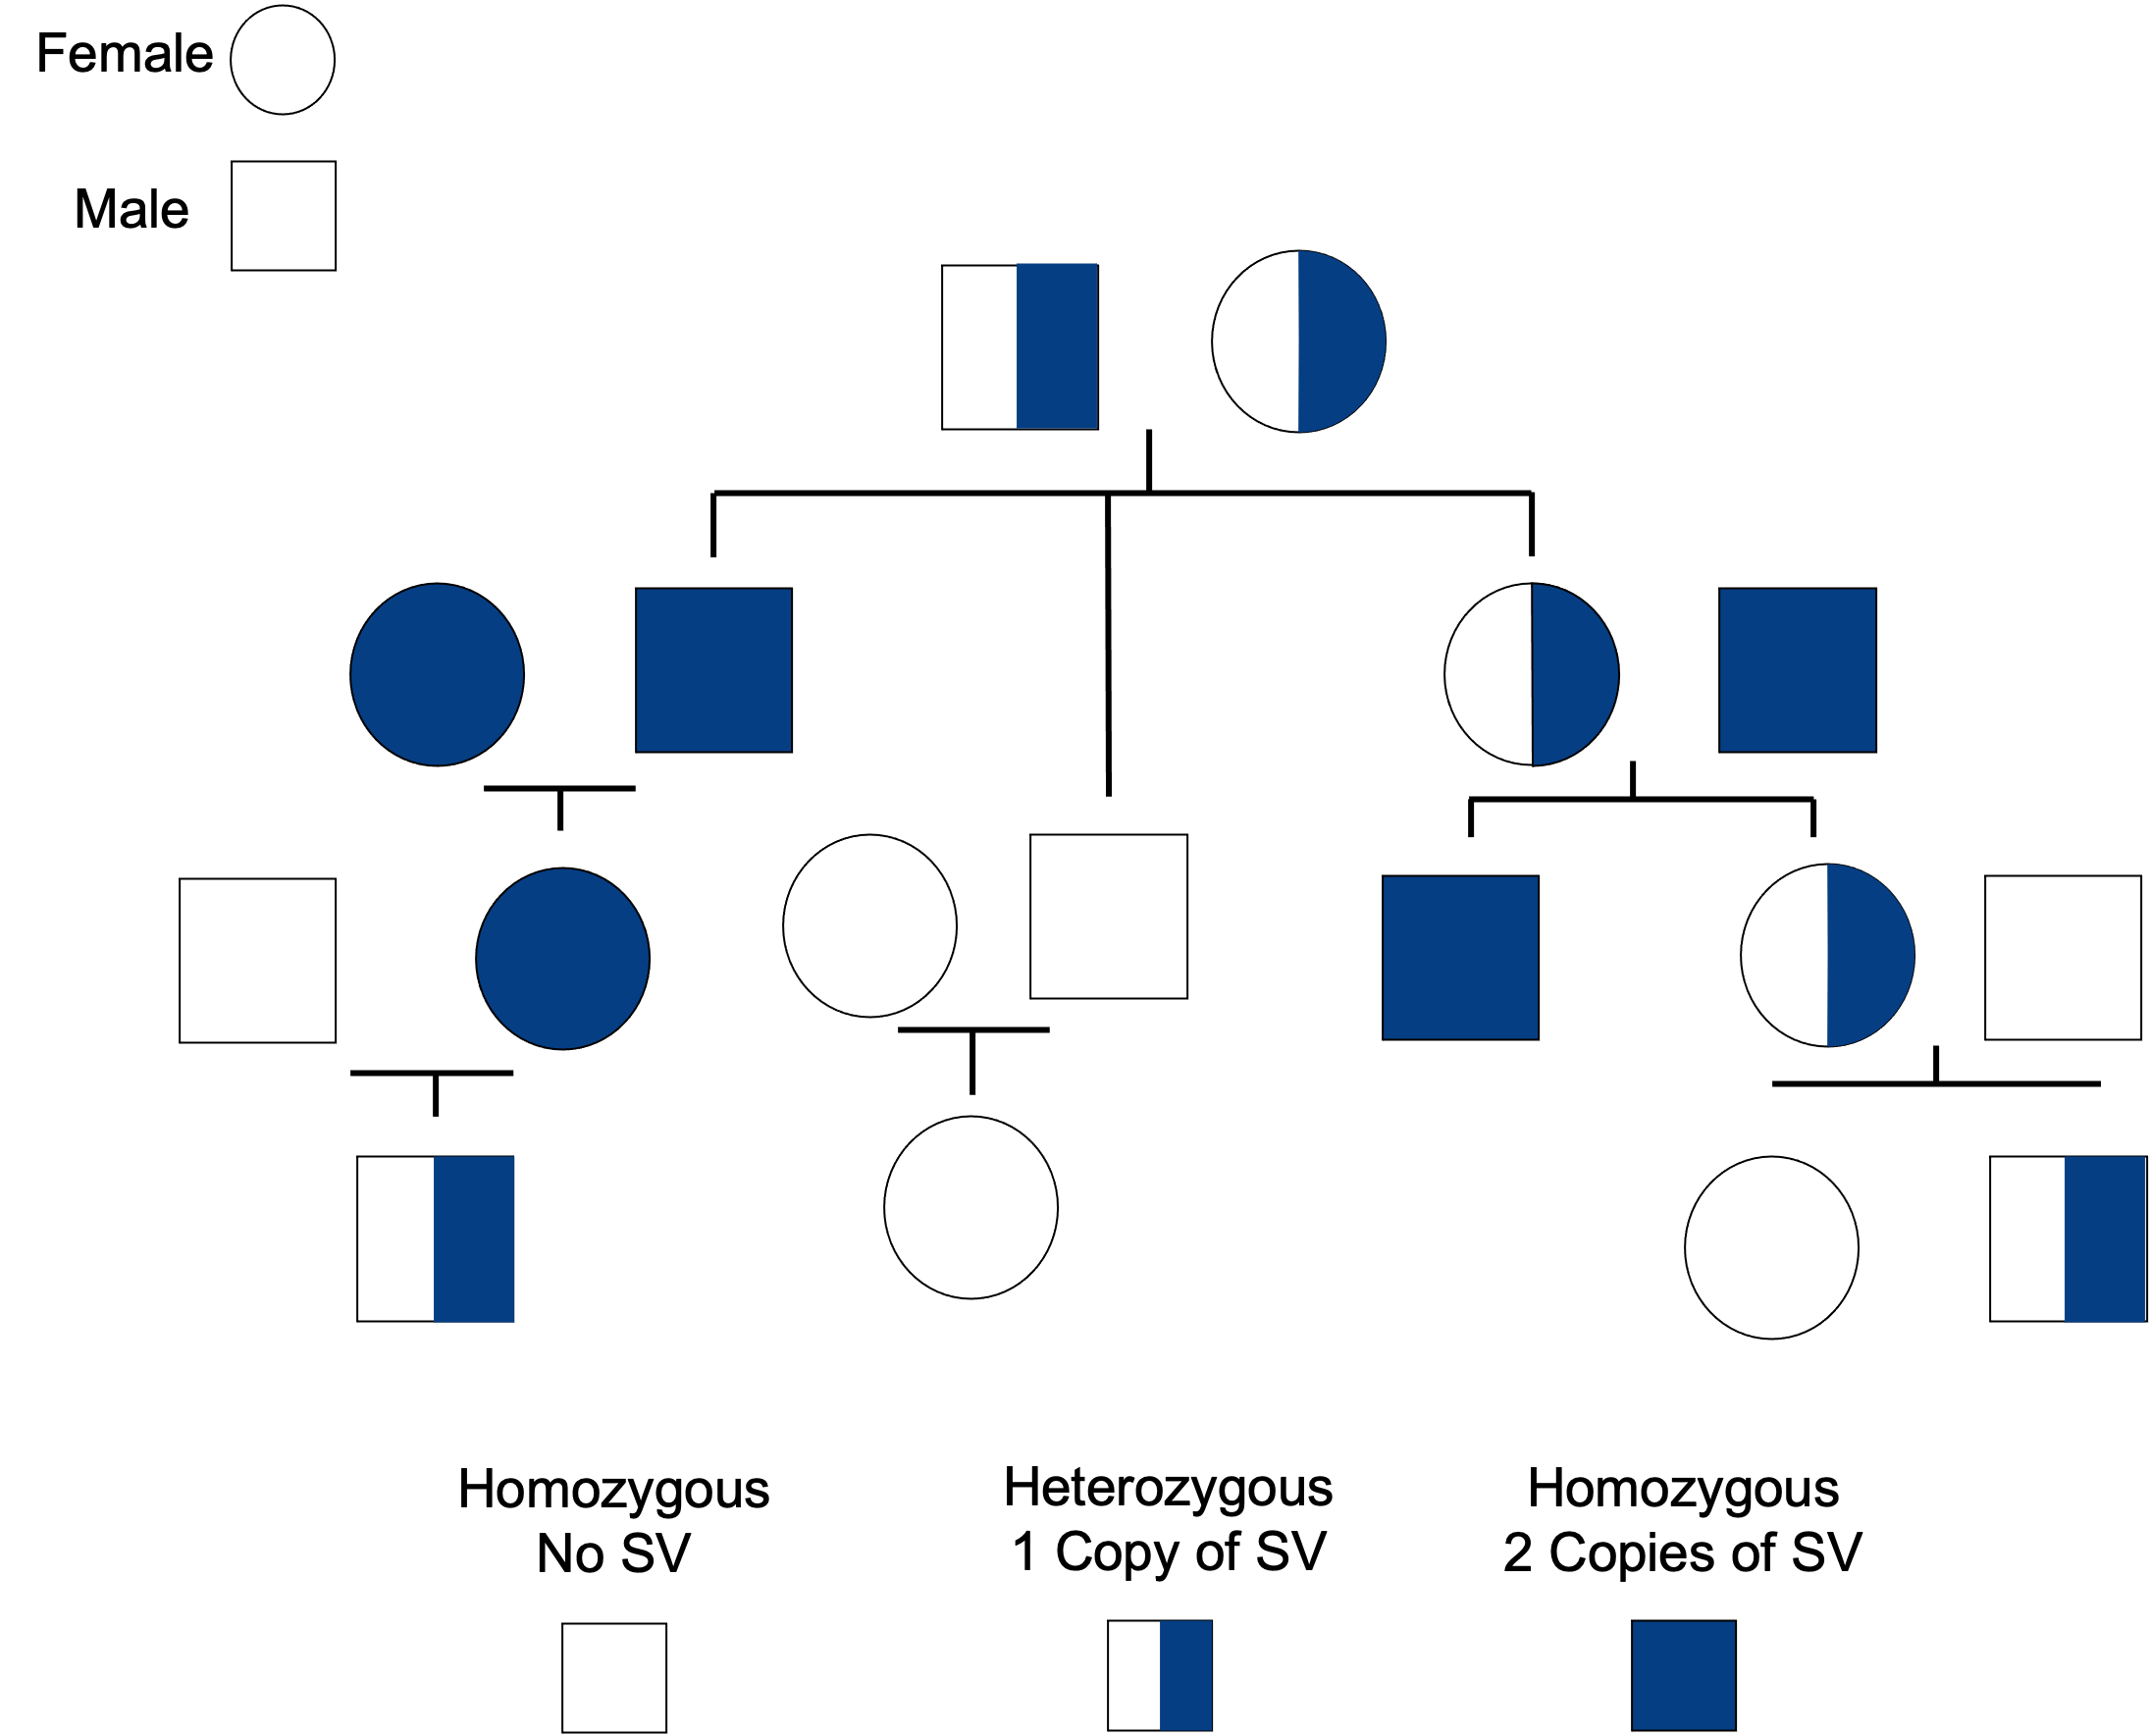
\includegraphics[width=6.0cm]{figs/familial_pedigree.png}}
%		%  \vspace{2.0cm}
%	\end{minipage}
%	\caption{Example of placing a figure with experimental results.}
%	\label{fig:res}
%	%
%\end{figure}

